\documentclass[twoside,10pt]{article}
\usepackage{amsmath,amsfonts,amsthm,fullpage,amssymb}
%\usepackage{mymath}
\usepackage{algorithm,amsmath,amssymb}
\usepackage{algorithmic}
\usepackage{graphicx, color}
\usepackage{url}


\begin{document}


\title{ISYE 6740 Homework 6 (Last Homework)\\ 
Fall 2023\\ 
\small Total 100 points}
\date{}
\maketitle



%As usual, please submit a report with sufficient explanation of your answers to each the questions, together with your code, in a zip folder.

%----------------------------------------------------------------------------------

%feature selection (CV, bias-variance tradeoff), Boosting, random forest 

\begin{enumerate}


\item {\bf Conceptual questions.} (20 points)

\begin{enumerate}

\item (5 points) Explain how we control the data-fit complexity in the regression tree. Name at least one hyperparameter that we can turn to achieve this goal.

\item (5 points) Explain how OOB errors are constructed and how to use them to understand a good choice for the number of trees in a random forest. Is OOB an error test or training error, and why?

\item (5 points) What's the main difference between boosting and bagging? The random forest belongs to which type?

\item (5 points) Explain how to prevent overfit in CART?

\end{enumerate}


%\clearpage

\item  {\bf AdaBoost.} (20 points)

Consider the following dataset, plotted in the following figure. The first two coordinates represent the value of two features, and the last coordinate is the binary label of the data.
\begin{equation*}
\begin{split}
&X_1 = (-1, 0, +1), X_2 = (-0.5, 0.5, +1), X_3 = (0, 1, -1), X_4 = (0.5, 1, -1), \\
&X_5 = (1, 0, +1), X_6 = (1, -1, +1), X_7 = (0, -1, -1), X_8 = (0, 0, -1).
\end{split}
\end{equation*}

In this problem, you will run through $T = 3$ iterations of AdaBoost with decision stumps (as explained in the lecture) as weak learners.

\begin{enumerate}
\item (10 points) For each iteration $t = 1, 2, 3$, compute $\epsilon_t$, $\alpha_t$, $Z_t$, $D_t$ by hand (i.e., show the calculation steps) and draw the decision stumps on the figure (you can draw this by hand). 

\item (10 points) What is the training error of this AdaBoost? Give a short explanation for why AdaBoost outperforms a single decision stump.

\end{enumerate}


%\vspace{-.2in}
\begin{figure}[h!]
\begin{center}
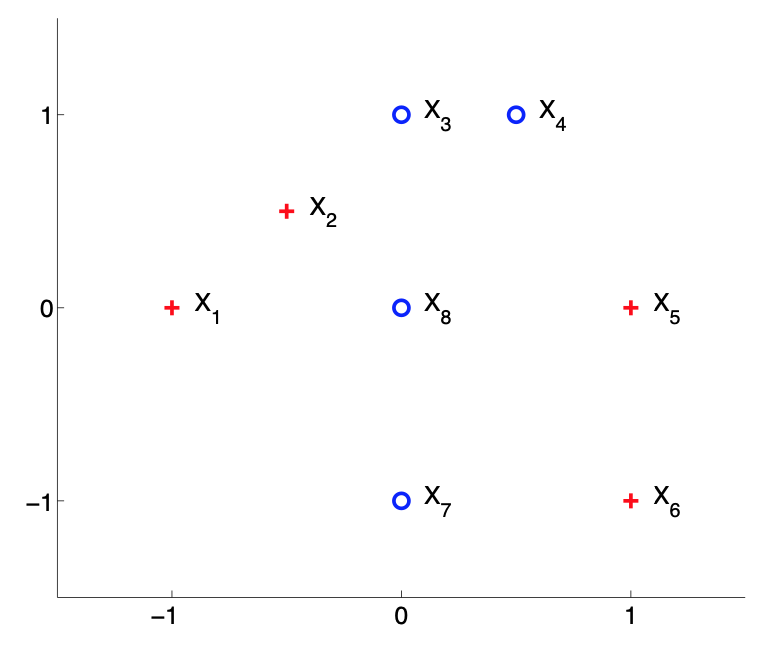
\includegraphics[width =.5 \textwidth]{hw}
\end{center}
\caption{ A small dataset for binary classification with AdaBoost.}
\end{figure}
%\vspace{-.3in}

\begin{table}
\begin{center}
\caption{Values of AdaBoost parameters at each timestep.}
\vspace{0.1in}
\begin{tabular}{|c|c|c|c|c|c|c|c|c|c|c|c|}\hline
t & $\epsilon_t$ & $\alpha_t$ & $Z_t$ & $D_t(1)$ & $D_t(2)$ & $D_t(3)$ & $D_t(4)$ & $D_t(5)$ & $D_t(6)$ & $D_t(7)$ & $D_t(8)$ \\\hline
1 & & & & & & & & & & & \\
2 & & & & & & & & & & &\\
3 & & & & & & & & & & & \\\hline
\end{tabular}
\end{center}
\end{table}

\clearpage

\item {\bf Random forest and one-class SVM for email spam classifier} (30 points)

Your task for this question is to build a spam classifier using the UCR email spam dataset \url{https://archive.ics.uci.edu/ml/datasets/Spambase} came from the postmaster and individuals who had filed spam. Please download the data from that website. The collection of non-spam emails came from filed work and personal emails, and hence the word \textsf{'george'} and the area code \textsf{'650'} (Palo Alto, CA) are indicators of non-spam. These are useful when constructing a personalized spam filter. You are free to choose any package for this homework. Note: there may be some missing values. You can just fill in zero.

\begin{enumerate}

\item (5 points) Build a CART model and visualize the fitted classification tree.

\item (5 points) Now, also build a random forest model. Randomly shuffle the data and partition to use  80\% for training and the remaining 20\% for testing. Compare and report the test error for your classification tree and random forest models on testing data. Plot the curve of test error (total misclassification error rate) versus the number of trees for the random forest, and plot the test error for the CART model (which should be a constant with respect to the number of trees). 


\item (10 points) Fit a series of random-forest classifiers to the data to explore the sensitivity to the parameter $\nu$ (the number of variables selected at random to split). Plot both the OOB error as well as the test error against a suitably chosen range of values for $\nu$.

\item (10 points) Now, we will use a one-class SVM approach for spam filtering. Randomly shuffle the data and partition to use  80\% for training and the remaining 20\% for testing. Extract all {\it non-spam} emails from the training block (80\% of data you have selected) to build the one-class kernel SVM using RBF kernel (you can turn the kernel bandwidth to achieve good performance). Then apply it to the 20\% of data reserved for testing (thus, this is a novelty detection situation), and report the total misclassification error rate on these testing data. 

\end{enumerate}

\clearpage 

\item {\bf Locally weighted linear regression and bias-variance tradeoff.} (30 points)

Consider a dataset with $n$ data points $(x_i, y_i)$, $x_i \in \mathbb R^p$, following the following linear model
\[
y_i = {\beta^*}^T x_i + \epsilon_i, \quad i = 1, \ldots, n,
\]
where $\epsilon_i \sim \mathcal N(0, \sigma^2)$ are i.i.d. Gaussian noise with zero mean and variance $\sigma^2$.

 
\begin{enumerate}

\item (5 points) Show that the ridge regression, which introduces a squared $\ell_2$ norm penalty on the parameter in the maximum likelihood estimate of $\beta$ can be written as follows
\[
\hat \beta (\lambda) = \arg \min_{\beta} 
\left\{
\|X \beta - y\|_2^2 + \lambda \|\beta\|_2^2
\right\}
\]
for property defined matrix $X$ and vector $y$. 


\item (5 points) Find the close-form solution for $\widehat {\beta}(\lambda)$ and its distribution conditioning on $\{x_i\}$.

\item (5 points) Derive the bias as a function of $\lambda$ and some fixed test point $x$.

\item (5 points) Derive the variance term as a function of $\lambda$.

\item (5 points) Now assuming the data are one-dimensional, the training dataset consists of two samples $x_1 = 0.15$ and $x_2 = 1.1$,  and the test sample $x = 1$. The true parameter $\beta_0^* = -1$, $\beta_1^* = 1$, the noise variance is given by $\sigma^2 = 0.5$. Plot the MSE (Bias square plus variance) as a function of the regularization parameter $\lambda$. 

\item (5 points) Now change the test sample to be a $x=1.5$, and keep everything else to be the same as in the previous question. Plot the MSE (Bias square plus variance) as a function of the regularization parameter $\lambda$, and comment on the difference from the previous result. 



\end{enumerate} 




\end{enumerate}





\end{document}
